% ================================================================
% TEMPLATE TRABALHO - DISCIPLINA DE EQUAÇÕES DIFERENCIAIS
% ================================================================
% IMPORTANTE:
% 1. Edite este arquivo e capitulo01.bib para colocar as referências.
% - Não altere o preâmbulo deste arquivo.
% - Não coloque \documentclass, \begin{document} ou \end{document}
% - Não altere a estrutura do arquivo na parte de referencias \printbibliography 
% ================================================================

\ifdefined\LivroPrincipal
  % --------------------------------------------------------------
  \chapter{TÍTULO DO TRABALHO}
  \newcommand{\FinalizaCapitulo}{}
\else
  % --------------------------------------------------------------
  % MODO AUTÔNOMO: permite ao grupo compilar este arquivo sozinho.
  % --------------------------------------------------------------
  \documentclass[11pt,a4paper]{article}

  \usepackage[utf8]{inputenc}
  \usepackage[T1]{fontenc}
  \usepackage[brazil]{babel}
  \usepackage{lmodern}
  \usepackage{microtype}
  \usepackage{amsmath,amssymb,amsfonts,amsthm,mathtools}
  \usepackage{bm}
  \usepackage{physics}
  \usepackage{siunitx}
  \usepackage{graphicx}
  \usepackage{booktabs}
  \usepackage{array}
  \usepackage{multirow}
  \usepackage{float}
  \usepackage{caption}
  \usepackage{subcaption}
  \usepackage{enumitem}
  \usepackage{xcolor}
  \usepackage{url}
  \usepackage{hyperref}
  \usepackage{cleveref}
  \usepackage{geometry}
  \usepackage{setspace}
  \usepackage{tikz}
  \usepackage{csquotes}
  \usepackage[backend=biber,style=numeric,sorting=nyt,maxbibnames=99]{biblatex}

  \geometry{left=2.8cm,right=2.3cm,top=2.5cm,bottom=2.5cm}
  \setstretch{1.08}
  \hypersetup{colorlinks=true,linkcolor=blue,citecolor=blue,urlcolor=blue}
  \newenvironment{resumo}{\begin{center}\textbf{Resumo}\end{center}\small}{\par}\normalsize
  \addbibresource{Referencias.bib} %alterar na entrega
  \newcommand{\FinalizaCapitulo}{\end{document}}

  \begin{document}
  \section*{Simulação de lançamento de foguete}
  \begin{center}
  Vinícius Marianno de Marque Cutolo; Pedro Lucas Miranda da Silva de Sá; Filipi Martins.
  \end{center}
\fi

\begin{resumo}
Apresente aqui, em aproximadamente 100--200 palavras, o problema estudado, o objetivo do trabalho, a metodologia utilizada, os principais resultados e a principal conclusão. Evite citações, equações longas e informações que não sejam retomadas no texto.
\end{resumo}

\noindent\textbf{Palavras-chave:} equações diferenciais; modelagem matemática; aplicações; simulação física; aeroespacial.

\section{Introdução}
A saída do planeta terra é o primeiro passo para a exploração espacial, com isso motivação do grupo é investigar o lançamento de um foguete para entrada na orbita do planeta terra, os problemas são modelar a atmosfera para determinar os efeitos dinâmicos em cada altura, e assim por fim modelar a dinâmica do foguete. O objetivo do trabalho é criar uma simulação que utilize os modelos criados, utilizado o foguete saturno V como base. % Apresente o problema, sua motivação e sua relevância. Explique claramente qual pergunta ou fenômeno será investigado, indique o objetivo do trabalho e contextualize a aplicação escolhida. O trabalho deve ter no \textbf{máximo 8 páginas}.

\section{Fundamentação teórica}
Apresente os conceitos matemáticos necessários para compreender o trabalho. Inclua as equações diferenciais utilizadas, hipóteses, definições, resultados teóricos, métodos analíticos e/ou numéricos e referências bibliográficas pertinentes. Toda afirmação ou resultado obtido de uma fonte externa deve ser devidamente referenciado, por exemplo~\cite{exemplo-livro}.

\subsection{Formulação matemática}

\subsubsection{Gravidade}

Pela lei da gravitação universal de Newton, a gravidade é modelada como \eqref{eq:grav_newton}.

\begin{equation}
  g(h)=\frac{G M}{r^2}
  \label{eq:grav_newton}
\end{equation}

Como a variável principal desse trabalho (a altura h) é em relação a superfície, a gravidade será convertida para a um equivalente, como na Equação~\eqref{eq:grav_red}.

\begin{equation}
  g(h)=\frac{G M}{(R+r)^2}
  \label{eq:grav_red}
\end{equation}

Isso significa que a gravidade na superfície é dada por \(h=0\), o que resulta em uma constante que será chamada de \(g_0\). Com isso, é possível converter \(g_0\) em \(g(h)\) multiplicando a equação por \((\frac{R}{R+h})^2\), resultando na formula \eqref{eq:grav}.

\begin{equation}
  g(h)=g_0(\frac{R}{R+h})^2
  \label{eq:grav}
\end{equation}

\subsubsection{Temperatura}

Segunda a atmosfera padrão \cite{LBL_StandardAtmosphere}, a atmosfera pode ser separada em camadas com regimes próprios de temperatura. Segundo ela, cada uma dessas estratificações segue o modelo linear proposto em \eqref{eq:temp_lin}.

\begin{equation}
  T(h) = C + \beta(h-h')
  \label{eq:temp_lin}
\end{equation}

Para descobrir a temperatura em cada ponto, o ideal seria integrar a equação de modo \(T(h)=C+\int_{0}^{h_f}\beta dh\). Contudo, para simplificar o modelo, a soma foi discretizada, resultando na Equação~\eqref{eq:temp}.

\begin{equation}
  T(h)=T_0+ \sum_{j=0}^{i-1} \beta_j\,(h_{j+1}-h_j) + \beta_i\,(h-h_i), \qquad h_i<h<h_{i+1}
  \label{eq:temp}
\end{equation}

Em que os valores de \(h_i\) e \(\beta_i\) são tabelados e podem ser encontrados em \cite{LBL_StandardAtmosphere}.

\subsubsection{Densidade}

Para a densidade, usou-se uma lógica de equilíbrio. Suponha que uma camada muito fina, de tamanho \(dh\), está estática dentro da atmosfera (equilíbrio hidrostático), isso significa que as forças nessa camada precisam gerar uma resultando zero. Logo, o peso da camada com a pressão inferior e a pressão superior precisam seguir a Equação~\eqref{eq:equi_atmo}.

\begin{equation}
  P(h)A - \rho g(h) A dh - P(h+dh)A=0
  \label{eq:equi_atmo}
\end{equation}

Com isso, cortando as áreas e aplicando o limite de \(dh\to 0\), obtemos a equação \eqref{eq:dif_atmo}.

\begin{equation}
  \frac{dP}{dh} = -\rho(h)g(h)
  \label{eq:dif_atmo}
\end{equation}

Admitindo os gases atmosféricos como ideias, ele podem seguir a equação de Clapeyron. Passando o volume dividindo e manipulando os seus termos, é obtido uma equação alternativa na forma \(P=\frac{\rho R_g T}{M_M}\), com isso, pode-se substituir o P em \eqref{eq:dif_atmo} e, ao manipular a equação e isolar \(d\rho\) obtém-se a Equação~\eqref{eq:dif_den}.

\begin{equation}
  \frac{d\rho}{dh}=-\rho(h)[\frac{g(h)M_M}{R_g T(h)}+\frac{1}{T(h)}\frac{dT}{dh}]
  \label{eq:dif_den}
\end{equation}

Essa equação possui solução analítica nas condições definidas de \(T(h)\). Aplicando o método de separação de variáveis, é possível integrar a equação e obter sua forma final exposta em \eqref{eq:den}.

\begin{equation}
  ln(\rho(h)) = -[
  \frac{R^2 g_0 M_m}{R_g}
  \cdot
  \frac{
  \beta(R+h)\ln\left(
  \frac{-\beta h_i+\beta h+C}{R+h}
  \right)
  +R\beta+\beta h_i-C
  }{
  (R+h)\left(\beta R+\beta h_i-C\right)^2
  }
  + ln(T(h)) + K_i]
  \label{eq:den}
\end{equation}

Para definir a constante \(K_0\), tomou-se como sabida a densidade a nível do mar. Para as outras constantes, sabe-se que não existem mudanças instantâneas entre dois pontos da atmosfera infinitamente próximos, logo, a constante foi ajustada para ser contínua entre fronteiras das camadas.

\subsubsection{Forças sobre a nave}

No total, quatro forças foram consideradas: peso, empuxo de Arquimedes, empuxo do motor e resistência do ar. A força peso saí instantaneamente ao aplicar a gravidade na massa, por isso, não é necessária de se desenvolver. O empuxo de Arquimedes, durante os testes, se mostrou desprezível perante as outras forças, por isso, não será muito comentado também, sua formula é resultado da pressão exercendo força contra o espaço delimitado por um objeto, sendo representada como \(E_y=\rho(h)g(h)v\).

O empuxo do motor da nave é composto por duas partes: o momento ganho pela ejeção de combustível e o momento ganho pela expansão dele. Quando se queima o propulsor, ele é liberado como uma massa \(dm\) a uma velocidade \(\mu_e\) para baixo, isso resulta em um ganho instantâneo para a nave de \(dm\mu_e\). Com isso, \(dQ=dm\mu_e\). Diferenciando ambas as partes no tempo, a Equação~\eqref{eq:combus} é obtida.

\begin{equation}
  F_e = \dot{m}\mu_e
  \label{eq:combus}
\end{equation}

Para a parte da expansão, os gases saem da câmara de combustão e expandem dentro do bocal para serem ejetados. Com isso, o gás saí com uma pressão \(P_e\), o que faz ele realizar uma força no ar abaixo do bocal. Considerando que o ar atmosférico puxa essa gás, a força da expansão pode ser escrita como \(\Delta P A_b\). Com isso, a força de empuxo do motor é dada pela Equação~\eqref{eq:emp_mot}.

\begin{equation}
  T = c(\dot{m}\mu_e+(P_e-P_a)A_b)
  \label{eq:emp_mot}
\end{equation}

A variável \(c\) seria uma variável de correção do angulo da chama, mas, por falta de tempo, acabou não sendo utilizada.

Por fim, a nave pode ser simplificada para um cilindro se deslocando em relação a partículas estáticas na atmosfera. A cada colisão, a nave transfere uma quantidade de momento \(dQ\) para a partícula, fazendo elas variarem uma quantidade . Então, em um tempo \(dt\) a nave varre um volume \(dV = A v dt\), o que faz ela colidir com \(dm_t = \rho(h)dV=\rho(h)A v dt\). Isso causa uma variação \(\Delta u\) na velocidade das partículas, o que resulta em \(F=\rho(h)A v \Delta u\). Agora, suponha que esse \(\Delta u = \alpha v\) e que \(\alpha\) pode ser escrito como \(\frac{C_D}{2}\). Isso resulta na Equação~\eqref{eq:arras}.

\begin{equation}
  F_D = \frac{1}{2}C_D \rho(h)A v^2
  \label{eq:arras}
\end{equation}

Defina as variáveis, parâmetros, condições iniciais ou de contorno e apresente o modelo matemático, como o apresentado na Equação~\eqref{eq:pvi}
\begin{equation}
\frac{dy}{dt}=f(t,y), \qquad y(t_0)=y_0.
\label{eq:pvi}
\end{equation}

Empuxo de arquimedes:

\[E_y=\rho(h)g(h)v\]

- \(\rho\): Densidade da camada atual

- \(g\): gravidade na camada atual

- \(v\): volume do foguete

Arrasto da nave:

\[F_D=-\frac{1}{2}C_D\rho(h)A|v|\vec{v}\]

- \(C_D\): Coeficiente de arrasto

- \(\rho\): Densidade da camada atual

- \(A\): Área efetiva do foguete

- \(v\): Velocidade do foguete

Empuxo do motor:

\[T= c( \dot{m} \mu_e + (P_e-P_a)A_e)\]

- \(c\): Coeficiente de correção do bocal

- \(\dot{m}\): Vazão de massa do bocal

- \(\mu_e\): Velocidade relativa dos gases na saída

- \(P_e\): Pressão de exaustão

- \(P_a\): Pressão atmosférica de saída

- \(A_e\): Área do bucal

As equações quando são acompanhadas de uma numeração, devem ser referenciadas em maiúsculo, isto é, deve-se utilizar Equação~\eqref{eq:pvi} ao invés de equação~\eqref{eq:pvi}. O mesmo vale para teoremas, proposições, lemas, corolários, definições, figuras e tabelas.


\subsection{Método de solução}
Descreva o método analítico ou numérico empregado. Quando pertinente, apresente algoritmo, discretização, critérios de erro e demais questões que sejam relevantes para o trabalho.

\section{Discussão dos resultados}
Apresente os resultados obtidos e discuta seu significado. Figuras e tabelas devem ser numeradas, possuir legenda e ser mencionadas no texto. Não se esqueçam que ao final da legenda sempre deve aparecer a fonte da figura, como pode ser visto na Figura~\eqref{fig:exemplo}.

Mantendo a vazão em $14000$ por todo o percurso nos leva até 344 km acima da superfície. 
Contudo, a saturno usou vazões distintas, então, copiando ele, temos $14000$ no primeiro estágio, $1000$ no segundo e 600 no terceiro (os gráficos ficam bem bonitos), dai, com isso, chegamos em 3000 km

\begin{figure}[H]
    \centering
    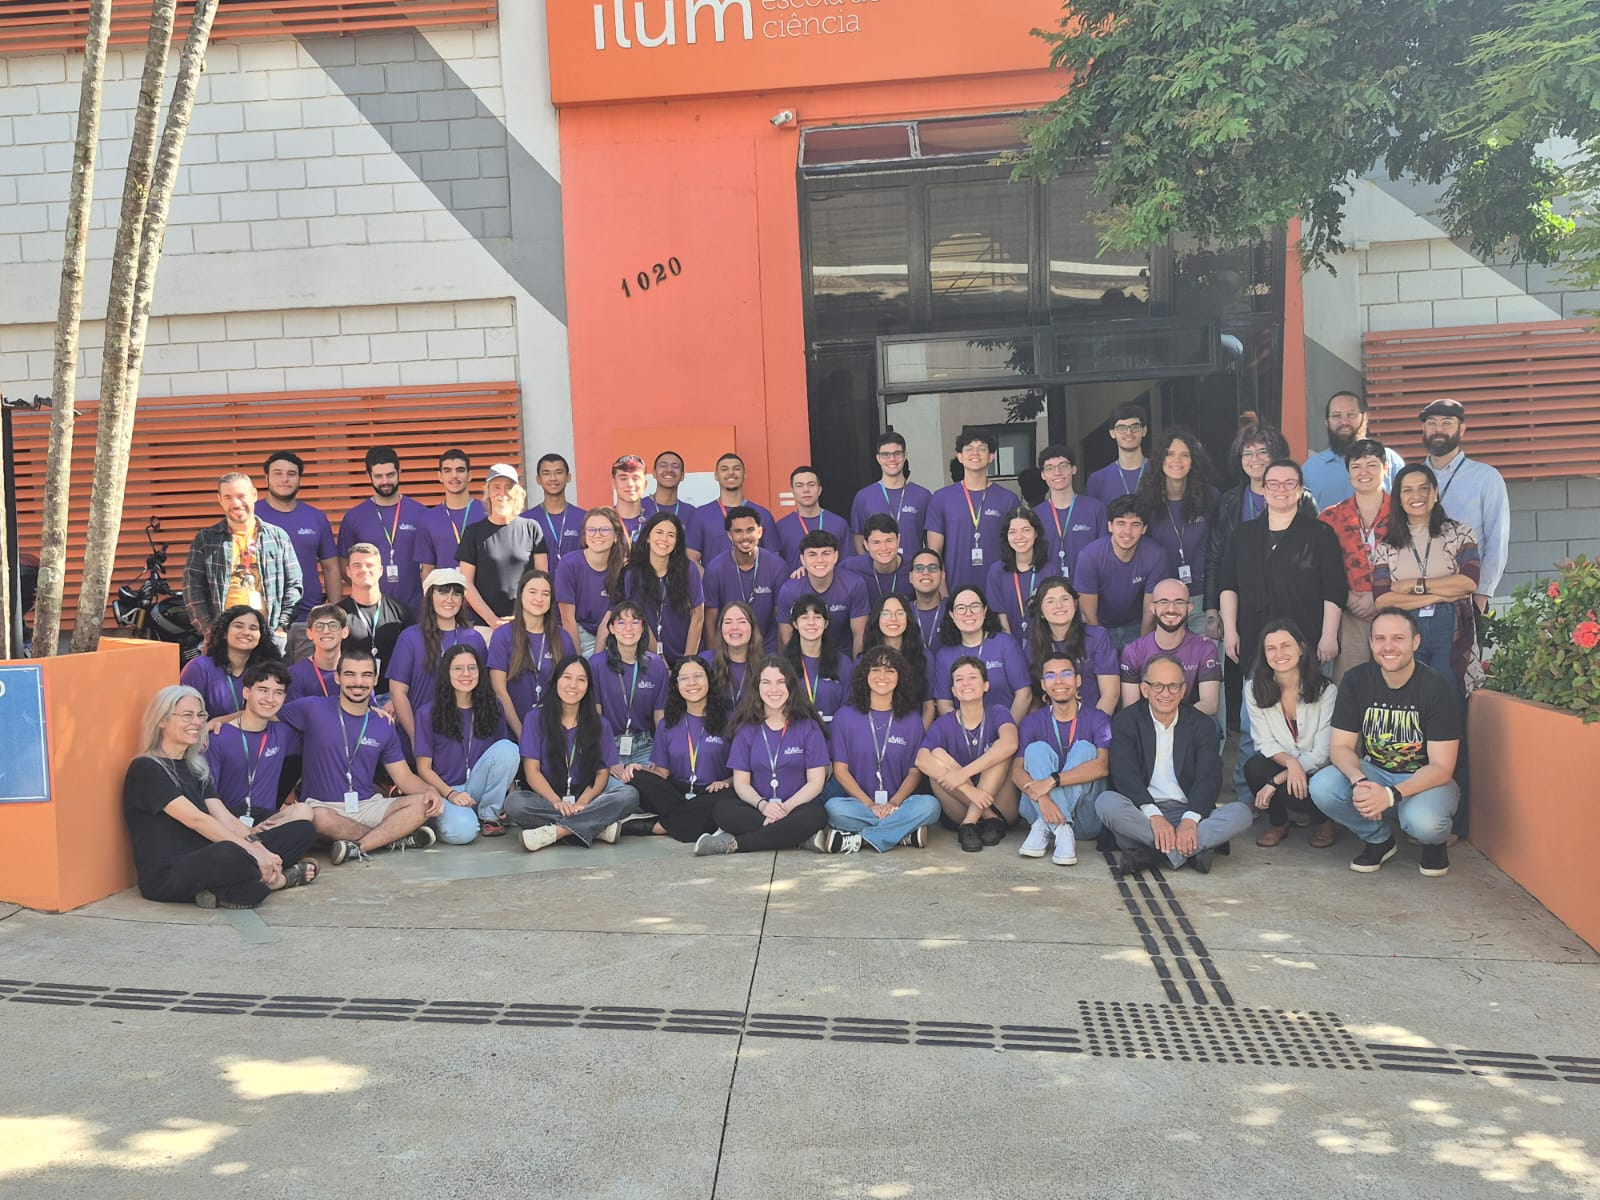
\includegraphics[width=0.9\linewidth]{Figures/t26.jpg}
    \caption{Turma 26 - Ilum Escola de Ciência. Fonte: Documentos oficiais da Ilum \url{https://ilum.cnpem.br/noticias_e_eventos/}}
    \label{fig:exemplo}
\end{figure}



Compare os resultados com a teoria, discuta limitações, comportamento do modelo, interpretações, erros de aproximação e demais informações relevantes para o trabalhos. Se for o caso, utilizem tabelas para auxiliar na organização da informação, como o modelo apresentado na Tabela~\ref{tab:exemplo}.

\begin{table}[H]
\centering
\caption{Exemplo de tabela.}
\label{tab:exemplo}
\begin{tabular}{lcc}
\toprule
Método & Erro & Tempo \\
\midrule
Método A & 0,00 & 0,00 \\
Método B & 0,00 & 0,00 \\
\bottomrule
\end{tabular}
\end{table}

\section{Considerações finais}
% Retome o objetivo do trabalho e apresente as principais conclusões. Destaque o que foi aprendido sobre o problema e sobre o uso de equações diferenciais na aplicação estudada. Não introduza resultados novos nesta seção. Perspectivas futuras são bem vindas, mas não obrigatórias.

\section{Contribuição de cada autor}
% Descreva objetivamente a participação de cada integrante. A descrição deve permitir identificar a contribuição individual de cada autor, incluindo, conforme o caso, revisão bibliográfica, formulação matemática, implementação computacional, análise dos resultados, produção de figuras e tabelas, redação e revisão do texto. \textbf{Utilizem essas informações para definir a ordem de autoria do trabalho}, isto é, a ordem deve ser da pessoa que mais contribuiu para aquela que menos contribuiu.

\begin{itemize}[leftmargin=*]
    \item Nome do Autor 1: descreva a contribuição.
    \item Nome do Autor 2: descreva a contribuição.
    \item Nome do Autor 3: descreva a contribuição.
\end{itemize}

% ================================================================
% Não altere esta parte.
% ================================================================
\ifdefined\LivroPrincipal
\else
  \printbibliography[heading=bibintoc,title={Referências}]
\fi
\FinalizaCapitulo

\end{document}